\documentclass[main.tex]{subfiles} % Subfile-Class

%==============================================================================%
%                                   Subfile                                    %
%==============================================================================%

\begin{document}

% Template

\section{Firmware GripController}~\label{apdx:FirmwareGripController}

Im folgenden Kapitel wird die Firmware des GripControllers näher beschrieben. Wie bereits im Hauptteil
erläutert, wurde die GripController Firmware als externe Komponente in die Firmware des MotionControllers
integriert. Durch diese Zusammenführung beider Firmwares sind nicht mehr alle Tasks der ursprünglichen
GripController Firmware erforderlich. Im folgenden Abschnitt werden dennoch alle vorhandenen Tasks kurz erläutert.

\subsection{ServoDriveTask}
Der ServoDriveTask steuert die State Machine für das Hindernishandling. Dabei prüft der Task in
regelmäßigen Abständen, ob ein neuer Befehl in der Queue eingetroffen ist oder ob der Notstopp
aktiviert wurde. Geht ein Befehl über die Queue ein, startet dieser die State Machine und leitet
den entsprechenden Ablauf ein. Ist hingegen der Notstopp aktiviert, wird der aktuelle Ablauf unterbrochen und 
bei erneuter aktivierung zurückgesetzt.\\
Nachdem der Befehl vollständig ausgeführt wurde, sendet der ServoDriveTask ein Acknowledge an die
MotionController Firmware und wartet anschliessend auf den nächsten Befehl.
\subsection{MotionControllerComTask}
Dieser Task dient dazu, UART-Befehle zu encodieren und zu versenden. Er stellt die Kommunikationsschnittstelle
zwischen dem MotionController-Print und dem GripController-Print dar. Da der GripController inzwischen in den
MotionController integriert wurde, verliert dieser Task an Bedeutung, da die Kommunikation nun intern erfolgt.
\subsection{TestTask}
Der TestTask simuliert einen unidirektionalen Informationsaustausch vom MotionController zum GripController.
Zu diesem Zweck wird zunächst ein „CraneGrip“-Befehl in die GripControllerRxQueue geschrieben. Nach einer
kurzen Wartezeit folgt ein „CraneRelease“-Befehl. Mithilfe dieser beiden Kommandos kann die State Machine
des ServoDriveTasks gestartet und unabhängig vom MotionController getestet werden. Auf das Testen des
„GcAck“ wird in diesem Task verzichtet.

\subsection{Ansteuerung des Greifmechanismus}
Der Greifer besteht aus zwei Servomotoren und zwei Endschaltern. Ein Servo ist für das Zugreifen zuständig,
der andere für das Hoch- und Herunterfahren des Greifers. Letzterer wird über die beiden Endschalter
positionsgenau gesteuert. Dadurch wird eine zuverlässige mechanische Positionsrückmeldung sichergestellt,
was insbesondere während der Entwicklung und Validierung für mehr Flexibilität und Sicherheit sorgte.\\
Damit die Servos bewegt werden können, wird ein PWM-Signal erzeugt, das den
gewünschten Winkel entsprechend anfährt. Der Servo, der für das Ergreifen des Hindernisses zuständig ist,
arbeitet dabei mit zwei fest definierten Winkelwerten. Der Servo für die Höhenverstellung wird hingegen in
mehreren kleinen Schritten angesteuert. Je nachdem, ob der Greifer nach oben oder nach unten fahren soll,
erfolgt die Winkelverstellung in positiven oder negativen Schritten. Die Schritte dienen als Verzögerung,
damit der Servo beim erreichen der Endschalter nicht überschiesst.\\
Die aktuelle Position des Greifers sowie der Status, ob ein Hindernis gegriffen wurde oder nicht, wird intern
über Status-Flags wie OBSTACLE\_GRIPPED oder SERVO\_OPEN verwaltet. Das gesamte Hindernishandling wird durch
eine State Machine gesteuert, welche die beiden Servos nacheinander entsprechend dem Ablauf ansteuert.

\subsection{Not-Aus-Verhalten}
Die Firmware überwacht kontinuierlich den Status des Not-Aus-Schalters. Im Falle einer Betätigung
wird die PWM-Ansteuerung beider Servomotoren deaktiviert. Ein gegebenenfalls laufender Greifvorgang wird dadurch unterbrochen.
Auf diese Weise kann ein unbeabsichtigtes Einklemmen durch den Greifer unterbrochen werden. Nach Freigabe des Notstopps kehrt das System automatisch
in die definierte Startposition zurück, wobei sich der Greifer geöffnet und in der oberen Endlage befindet. Die Position des Greifers, die
vor der Betätigung des Notstopps eingenommen wurde, ist in diesem Zusammenhang nicht mehr relevant.

\subsection{ServoDriveStm}
Die in Abbildung~\ref{fig:ServoDriveStm} dargestellte State Machine übernimmt die Steuerung des Ergreifens und Absetzens eines Hindernisses auf der Strecke.
Im folgenden Abschnitt wird der Ablauf der ServoDrive-Zustandsmaschine detaillierter erläutert.\\
Zu Beginn befindet sich die State Machine im \textit{IDLE} Zustand und erwartet dort einen gültigen Befehl von dem MotionController.
In Abhängigkeit des empfangengen Kommandos erfolgt eine Verzweigung in einen der beiden folgenden Zustände:
\textit{CRANE\_DOWN\_EMPTY} oder \textit{CRANE\_DOWN\_GRIPPED}.\\
Diese Unterscheidung wird bewusst vorgenommen, um eine zielgerichtete Steuerung der Zustandsmaschine zu ermöglichen.
Diese Aufteilung ermöglicht die mehrfachgie Auslösung des Greif- oder Absetzvorgangs. Im Falle einer erneuten Ausführung des selben
Befehls wird das entsprechende Statusflag \textit{OBSTACLE\_GRIPPED} zurückgesetzt. Der Ablauf lässt sich damit beliebig oft wiederholen,
ohne dass das System durch die Statusflags in einen blockierten Zustand versetzt wird.\\
Unabhängig davon, welcher Crane-Down-Zustand aktiv war, führt das Erreichen der unteren Endposition des Greifers
zum \textit{HANDLE\_OBSTACLE} Zustand. In diesem Zustand entscheidet das interne Statusflag, ob der Greifer geöffnet
oder geschlossen werden soll. Nach dem Abschluss des Greifvorgangs erfolgt der Übergang in den Zustand \textit{CRANE\_UP}.
In diesem Zustand ist es irrelevant, ob ein Hindernis gegriffen wurde oder nicht. Der Greifer fährt lediglich in die obere Endlage.
Beim Erreichen dieser Endlage wird ein GcAck-Befehl an die Firmware des MotionControllers übermittelt und in 
den Zustand \textit{IDLE} gewechselt. In diesem Zustand wartet die State Machine auf einen neuen Befehl.\\
Aus jedem Zustand kann durch die Betätigung des Not-Aus-Schalters unmittelbar in den Zustand \textit{STOP} gewechselt
werden. Sobald der Notstopp wieder freigegeben wird, kehrt die State Machine in den \textit{IDLE} Zustand zurück.


\begin{figure}[H]
    \centering
    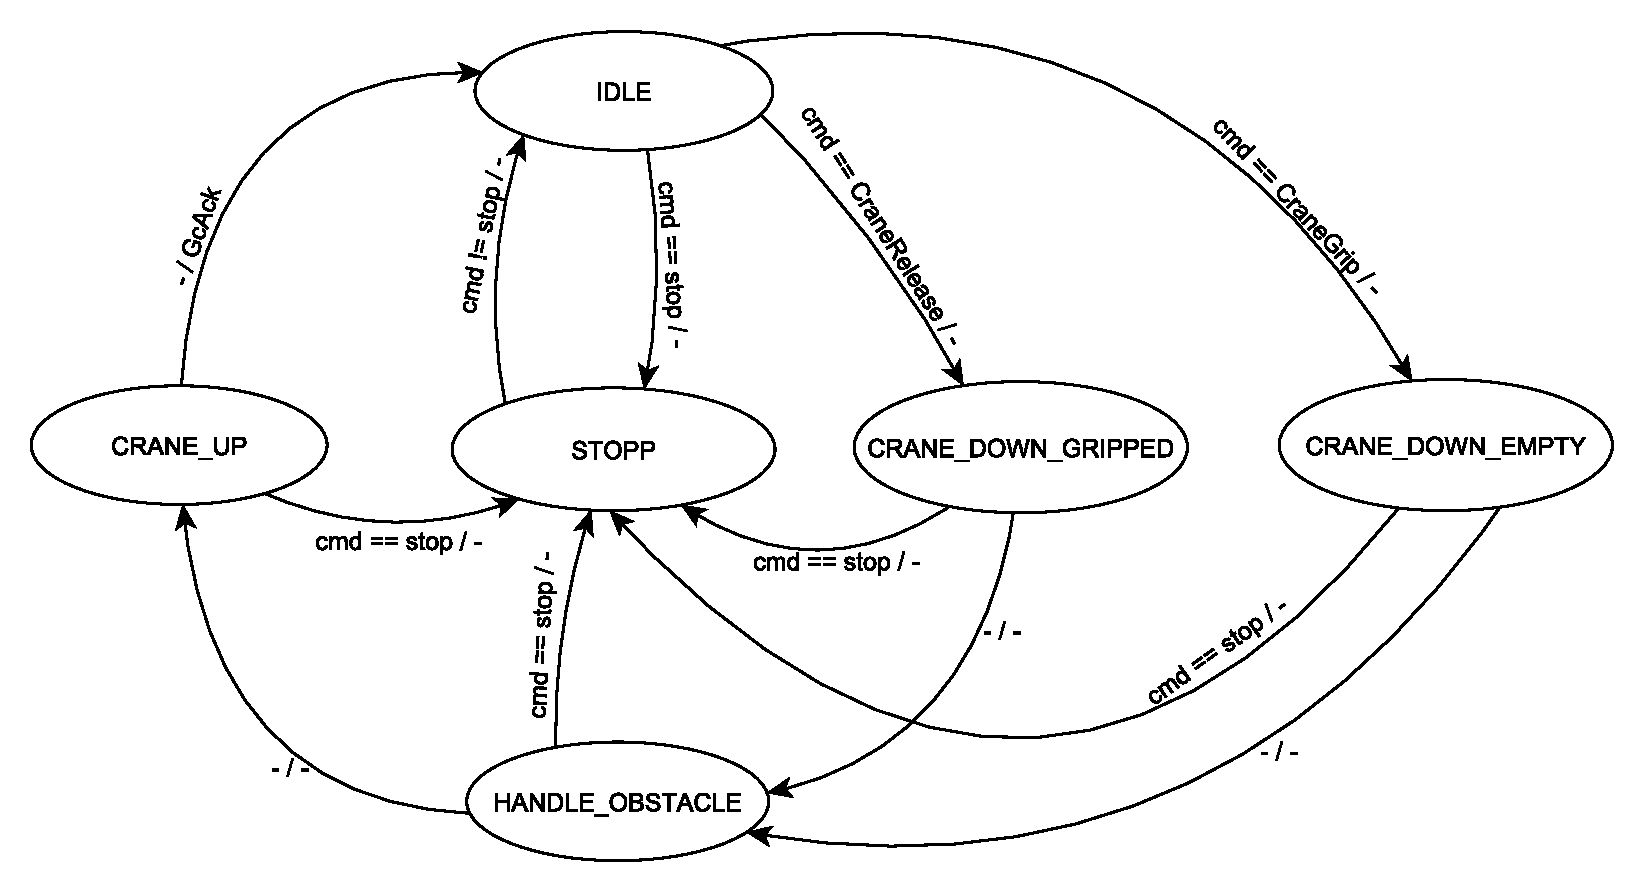
\includegraphics[width=1\linewidth]{./fig_Firmware_GripController/ServoDriveStm.pdf}
    \caption{Zustandsdiagramm ServoDriveStm}~\label{fig:ServoDriveStm}
\end{figure}



%- Wie ist GripController strukturiert
%- Wie werden Servos initialisiert
%- was gibt es für Kommandos
%- wie wird auf Stopp reagiert
%- ...

\end{document}
